\chapter{Pairing-Based Contact Discovery}
\label{chap:system}

\paragraph{} In this chapter we present the architecture for our contact discovery service (\autoref{sec:architecture}). We then provide outlines of security proofs (\autoref{sec:security}), theoretical performance evaluations (\autoref{sec:performance}) and show how our system maps onto real-world applications such as end-to-end encrypted messaging and mobile-first cryptocurrencies (\autoref{sec:applications}).


\section{Formal problem statement}
\label{sec:probstatement}

\paragraph{} First, we provide a formal definition for the problem of contact discovery. User $A$ is registered to a third-party application from which she receives an opaque account identifier $\acc_A$, an address $\addr_A$ and a secret/public key pair $(\sk_A,\pk_A)$. User $A$ also holds a human-readable discovery identifier $\id_A$ (mobile phone number or an email-address) and a list of contacts. We represent $A$'s address book as a set of discovery identifiers $\contacts{A}$. We assume that users exchanged discovery identifiers through out-of-bound communication but are unable to exchange cryptographic material, including their public keys. Thus for all users $B$ such that $\id_B \in \contacts{A}$ and $\id_A \in\ \contacts{B}$, $A$ wishes to learn the tuple $(\addr_B, \pk_B)$.

\section{Service architecture}
\label{sec:architecture}

\paragraph{} The foundational design principle for our contact discovery scheme is to provide users with the means to perform contact discovery locally. As we have seen in \autoref{chap:litreview}, sending a client the full list of registered users in a probabilistic data structures such as Bloom and Cuckoo filters requires the client to download and store large amounts of data. Instead, we follow an approach similar to the IBKE protocols. Our scheme runs in three phases which we will investigate individually:
\begin{enumerate}
	\item \textbf{Setup:} a one-time step for each user. During the setup phase, a user interacts with the contact discovery service to obtain her unique cryptographic material.
	\item \textbf{Key derivation:} using this cryptographic material, the user is able to compute shared secret keys with any of her contacts knowing only their discovery identifier.	\item \textbf{Discovery:} using their shared secret key, a pair of users can establish a secure meeting point on an untrusted online cache, thus allowing for asynchronous contact discovery.
\end{enumerate}

\noindent \autoref{fig:diagram} shows a diagram of the process described above.

\begin{figure}[H]
	\begin{center}	
	  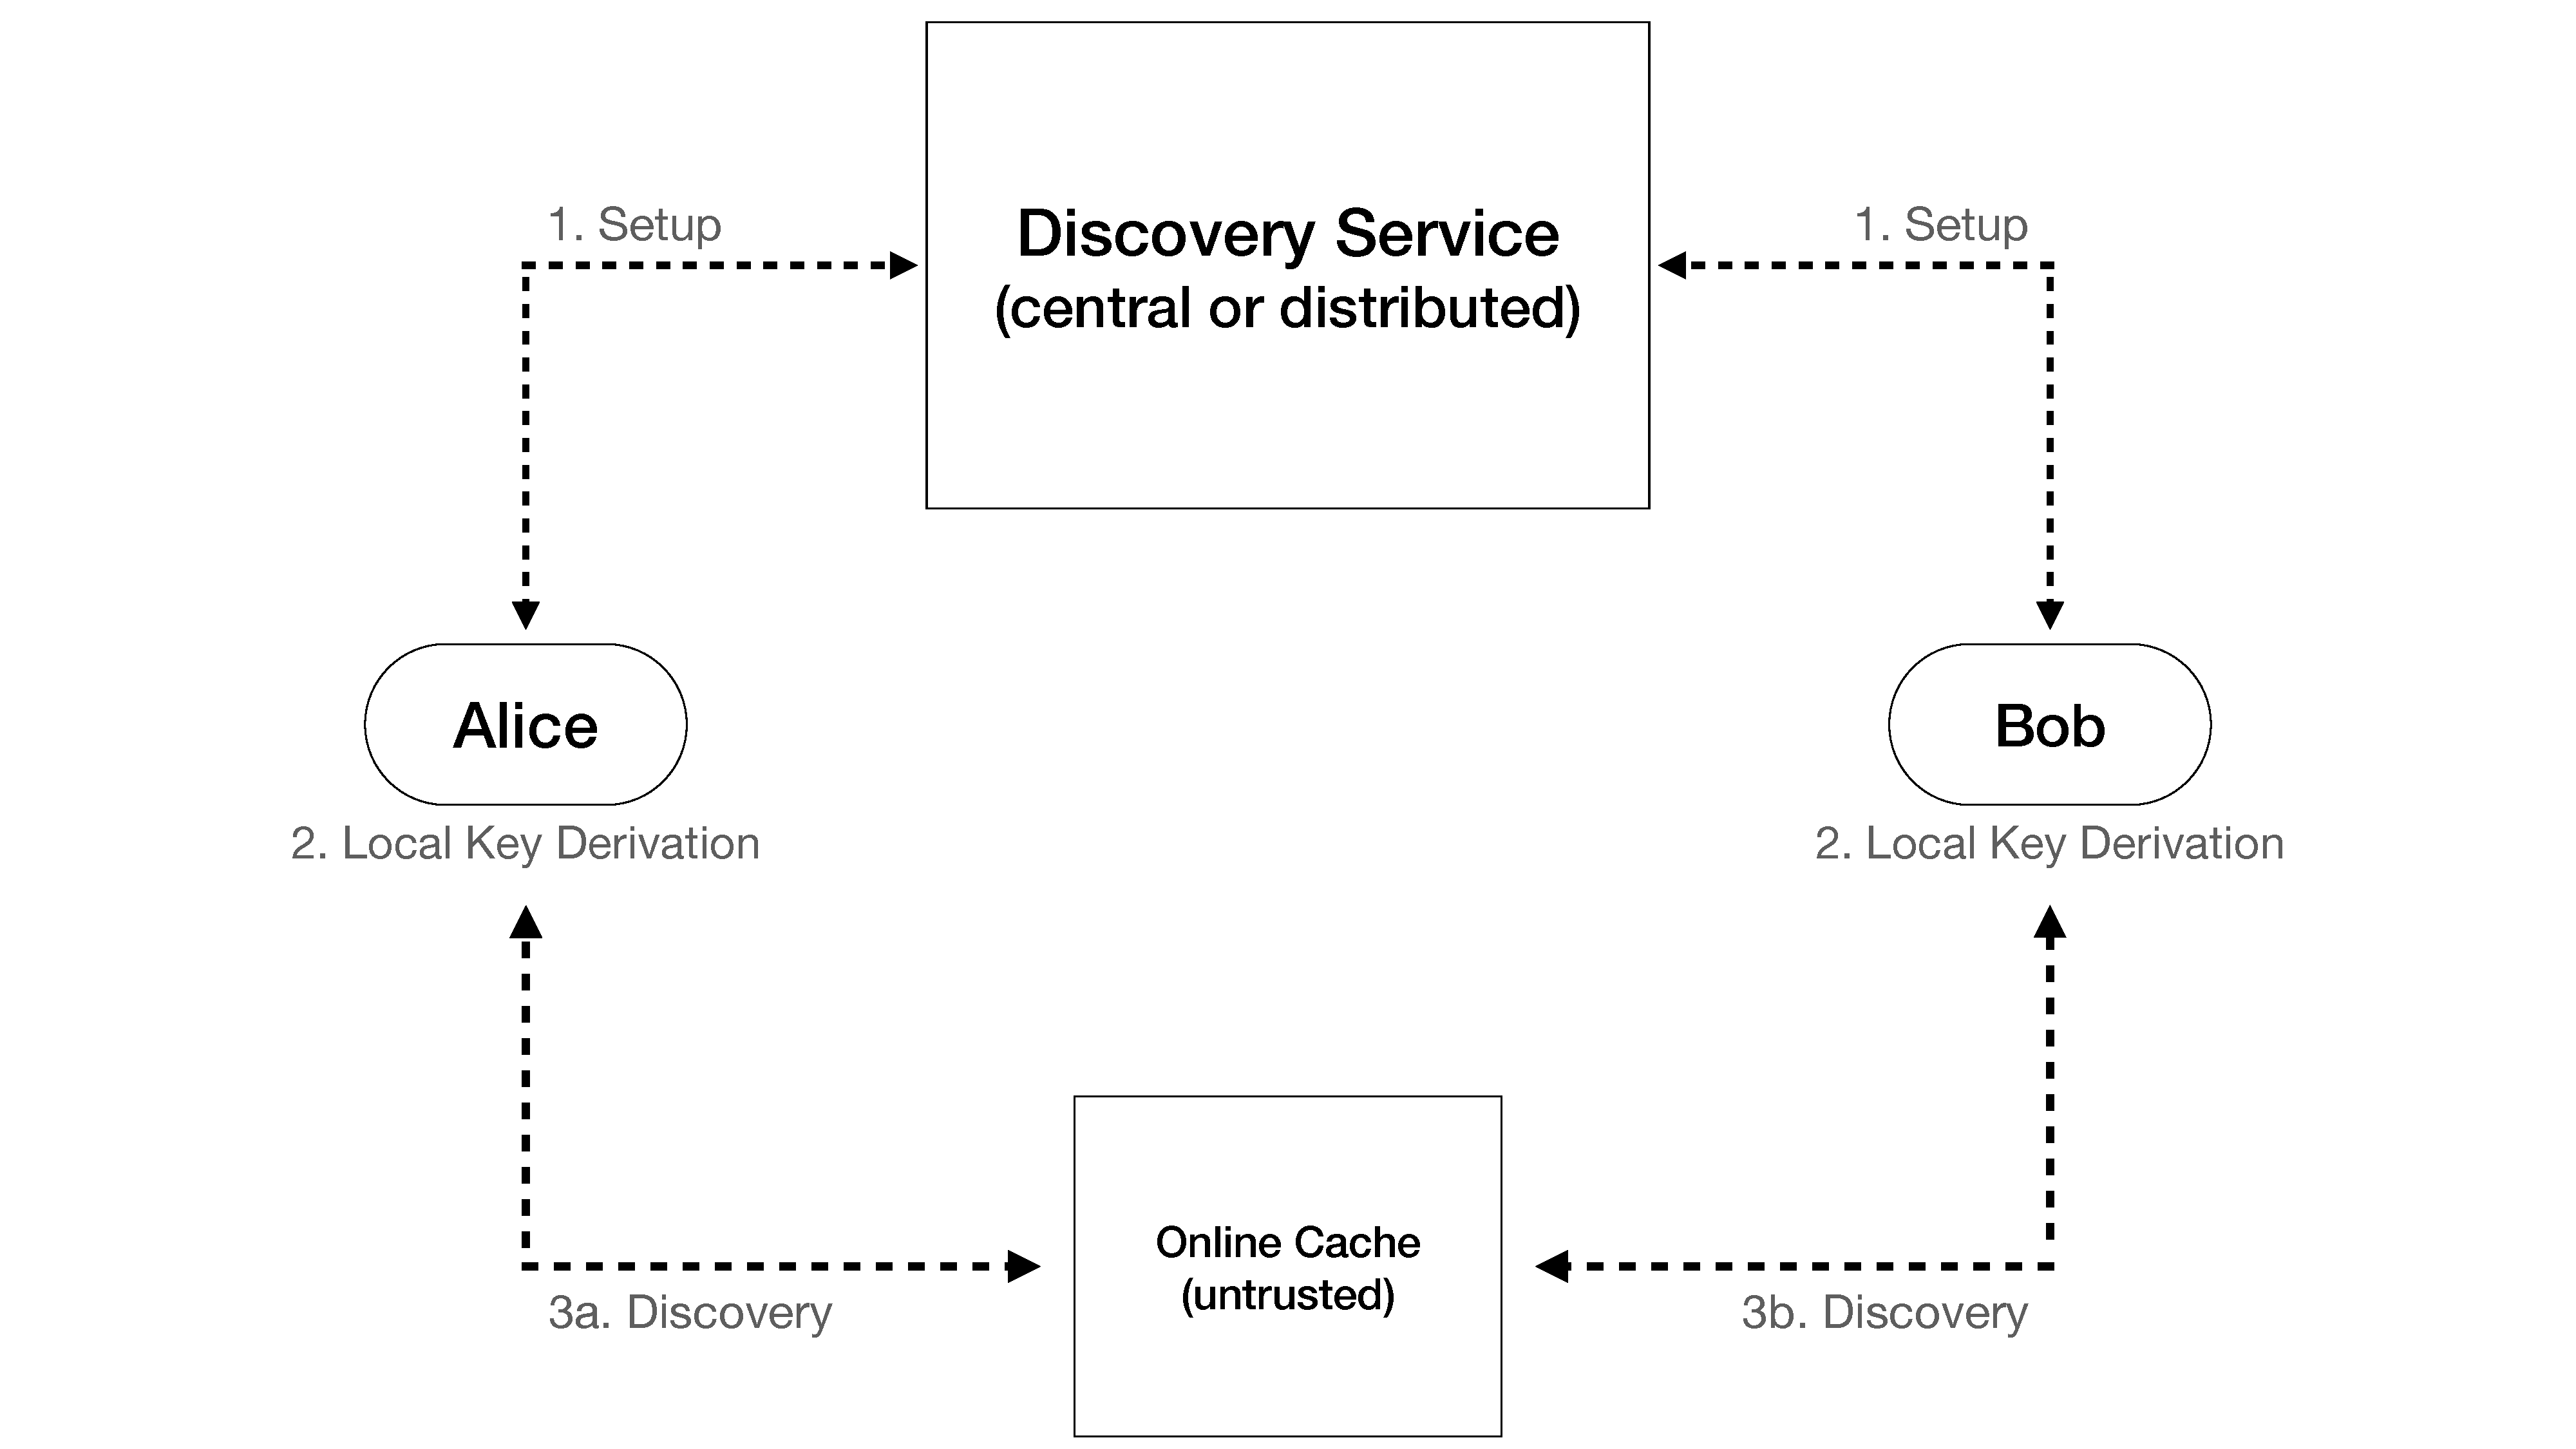
\includegraphics[width=\textwidth]{figures/system}
	  \caption{Contact discovery between a pair of users Alice and Bob, including setup. Numbers indicate the order of execution}
	  \label{fig:diagram}
	 \end{center}
 \end{figure}

	\subsection{Actors, assets and notation}
	
		\noindent We make a brief aside to clarify the actors and assets present in our scheme:		
		\begin{itemize}
			\item \textbf{Users:} each user $A$ holds an opaque account identifier $\acc_A$, an address $\addr_A$, a key pair $(\sk_A,\pk_A)$, a discovery identifier $\id_A$ and an address book $\contacts{A}$ (see \autoref{sec:probstatement}). We denote $\mathcal{ID}$ the set of all existing discovery identifiers.
			\item \textbf{Discovery Service:} the discovery service $S$ may be a central or distributed entity. In the centralised version, the discovery service holds a master secret key $\msk$. In the distributed version, we denote the set of all servers as $\mathcal{S}$ and the $i$-th server as $S_i$. Each server holds a share of the master secret key $\msk_i$. Furthermore, in both versions, each server holds a list of tuples $(\acc, \pk)$ for all registered users.
			\item \textbf{Online Cache:} the online cache may be operated by the discovery scheme or by a third party and is assumed to be untrusted. Its role is to manage key-value pairs.
			
			\end{itemize}
			
		\noindent Next we define the cryptographic setting for our scheme:
		\begin{itemize}
			\item $\Gzero, \Gone, \Gt$ are three cyclic groups of prime order $q$ such that there exists a pairing $e : \Gzero \times \Gone \rightarrow \Gt$.
			\item $H_0: \mathcal{ID}\rightarrow \Gzero$  and $H_1: \mathcal{ID} \rightarrow \Gone$ are two public hash functions modelled as random oracles.
			\item $F: \mathcal{ID}^2 \times \mathbb{Z}_q \rightarrow \Gt$ is a left/right constrained PRF defined as: \begin{equation}
				F(k, (\id_A, \id_B)) = F_k(\id_A, \id_B)= \Pair{H_0(\id_A)}{H_1(\id_B)}^k
			\end{equation}
			\item $\mathbf{KDF}$ is a public, deterministic key derivation function.
			\item $\Sign$ and $\Verif$ are the two algorithms of a probabilistic and secure signature scheme which makes use of the third-party provided user keys $(\sk_A,\pk_A)$ 
			\item The master secret key $\msk$ is set to an integer $s \in \mathbb{Z}_q$ chosen uniformly at random. We define two corresponding master public keys $\mpk_0 = {g_0}^s$ and $\mpk_1 = {g_1}^s$. In the distributed variant, we assume that the master secret key is shared according to a secure $t$-out-of-$n$ secret sharing scheme and that no single entity holds the master secret key.
		\end{itemize}

	\subsection{Key derivation}
	
		\paragraph{} We first introduce the essential key derivation step. In doing so, we provide the reader with the necessary material to understand the security constraints under which the initial setup phase operates.
		
		\paragraph{} For all users $B$ such that $\id_B \in \mathcal{C}_A$, user $A$ can compute shared key material with $B$ by evaluating $F_\msk(\id_A, \id_B)$ and $F_\msk(\id_B, \id_A)$. From the definition of left/right constrained PRFs, $A$ can do so with the constraining keys $\keyleft{\id_A}$ and $\keyright{\id_A}$:
		\begin{align}
			s_{AB} = F_\msk(\id_A, \id_B) &= \Pair{\keyleft{\id_A}}{H_1(\id_B)} \\
			s_{BA} = F_\msk(\id_B, \id_A) &= \Pair{H_0(\id_B)}{\keyright{\id_A}}
		\end{align} 
	
	\noindent Similarly, $B$ can evaluate $F$ at the same points using the constraining keys $\keyleft{\id_B}$ and $\keyright{\id_B}$:		
		\begin{align}
			s_{AB} = F_\msk(\id_A, \id_B) &= \Pair{H_0(\id_A)}{\keyright{\id_B}} \\
			s_{BA} = F_\msk(\id_B, \id_A) &= \Pair{\keyleft{\id_B}}{H_1(\id_A)} 
		\end{align}
	
\noindent Using this key material, $A$ and $B$ can establish a symmetric secret key using a standardised key derivation function:
	\begin{equation}
		k_{AB} = k_{BA} = \mathbf{KDF}\left(s_{AB} \xor s_{BA}\right)
	\end{equation}
	
	\paragraph{A note on security --} The constraining keys $\keyleft{\id_A}$ and $\keyright{\id_A}$ allow to compute every symmetric key that $A$ may establish with her contacts. As such, those \textbf{constraining keys must remain private} to $A$. The consequences of a leak range from impersonation to a total leak of $A$'s address book and are further detailed in \autoref{sec:security}.
	
	\subsection{Discovery}
	
		\paragraph{} Using their shared key material $(k_{AB}, s_{AB}, s_{BA})$, users $A$ and $B$ can determine secret memory locations on the online cache to leave an encrypted message for each other. Let $(\enc$, $\dec)$ be a secure symmetric encryption scheme and $H$ a hash function modelled as a random oracle, we define two cache operations $\mathbf{Write}$ and $\mathbf{Read}$:
		\begin{itemize}
			\item $\mathbf{Write}$: store the key-value pair $(H(s_{AB}), \enc_{k_{AB}}(\pk_A || \addr_A))$ on the online cache.
			\item $\mathbf{Read}$: retrieve the key-value pair $(H(s_{BA}), c_{BA})$. If $B$ has already run the discovery phase of our scheme then $c_{BA} = \enc_{k_{BA}}(\pk_B||\addr_B)$. Decrypt $c_{BA}$ using the key $k_{AB} = k_{BA}$.
		\end{itemize}
	
	\subsection{Setup}
	\label{sec:setup}
		
		\paragraph{}  The setup stage serves to provide user $A$ with the constraining keys $k_{\id_A,\mathrm{LEFT}}$ and $k_{\id_A,\mathrm{RIGHT}}$. Consequently, the setup is a security-critical task. As we have shown in \autoref{eq:constrkeys}, under our construction of $F$ the constraining keys can be expressed as:
		\begin{equation}
			k_{\id_A,\mathrm{LEFT}} = H_0(\id_A)^\msk \quad \mathrm{and} \quad k_{\id_A,\mathrm{RIGHT}} = H_1(\id_A)^\msk
		\end{equation}
		
		\noindent These constraining keys are equivalent to BLS signatures on $\id_A$ by the discovery service. Notice that the service needs to produce signatures under both variants of the BLS scheme: one with signatures in $\Gzero$ and one with signatures in $\Gone$.
				
		\paragraph{} The setup protocol in the centralised variant between user $A$ and the server $S$ is described as follows:
		\begin{enumerate}
			\item $A$ chooses a random blinding factor $\alpha \sample \mathbb{Z}_q$ and sends $\acc_A$, $\mathbf{sig}_A = \Sign(\sk_A, \acc_A)$, $H_0(\id_A)^\alpha$, $H_1(\id_A)^\alpha$ to $S$.
			\item Upon reception of $A$'s request, $S$ retrieves the associated public key and checks that the signature $\mathbf{sig_A}$ is valid:
			\begin{equation}
				\Verif(\pk_A, \acc_A, \mathbf{sig}_A) = 1
			\end{equation}
		\item If the check succeeds, $S$ sends $(H_0(\id_A)^\alpha)^\msk$ and $(H_1(\id_A)^\alpha)^\msk$ to $A$
		\item $A$ checks the following equalities:
		\begin{align}
			\Pair{(H_0(\id_A)^\alpha)^\msk}{g_0} &= \Pair{H_0(\id_A)^\alpha}{\mpk_0} \\
			\Pair{g_1}{(H_1(\id_A)^\alpha)^\msk} &= \Pair{\mpk_1}{H_1(\id_A)^\alpha}
		\end{align}
		\item If the checks succeed (in other words, if $A$ receives valid signatures from the service), $A$ removes the blinding factor $\alpha$ to obtain $H_0(\id_A)^\msk$ and $H_1(\id_A)^\msk$.
		\end{enumerate}
		
		
%\fbox{
%	\procedure{Setup}{%
%		\textbf{user } A  \< \<\textbf{server } S \\
%		\alpha \sample \mathbb{Z}_q \< \\
%		\mathbf{sig}_A = \Sign(\sk_A, \acc_A) \< \\
%		\<\sendmessageright{top={$\acc_A,\mathbf{sig}_A, H_0(\id_A)^\alpha, H_1(\id_A)^\alpha$} } \\
%		\<\< \text{If } \Verif(\pk_A, \acc_A, \mathbf{sig}_A) = 0 \\
%		\<\< \qquad\textbf{Abort}\\
%		\<\< \text{Else}\\
%		\< \sendmessageleft{top={$(H_0(\id_A)^\alpha)^\msk, (H_1(\id_A)^\alpha)^\msk$}} 
% }
% }
	
	\paragraph{} The distributed version of the setup protocol is almost identical in every way: $A$ interacts as above with each server $S_i$ to obtain shares of her constraining keys $H_0(\id_A)^{\msk_i}$ and $H_0(\id_A)^{\msk_i}$. With enough shares, $A$ can run the recover algorithm from the sharing scheme to compute $H_0(\id_A)^\msk$ and $H_1(\id_A)^\msk$.
	
	


\section{Security}
\label{sec:security}

	\subsection{Outlines of security proofs}

	\subsection{Consequences of a breach}
	
	\subsection{Authentication: an open problem}


\section{Theoretical performance evaluation}
\label{sec:performance}


\section{Applications}
\label{sec:applications}

	\subsection{End-to-end encrypted messaging}
	
	\subsection{Mobile-first cryptocurrencies}
